\documentclass[onecolumn, 12pt]{IEEEtran}
\usepackage{graphicx}
\usepackage{cite}
\usepackage{amsmath, amssymb}
\usepackage{url}
\usepackage{hyperref}

\title{SeatSurfer: An AI-Driven Architecture for Hybrid Workplace Booking and Smart Office Management}

\author{
    \IEEEauthorblockN{Radu-Matei Prodan }
    \IEEEauthorblockA{
        \textit{Faculty of Mathematics and Computer Science} \\
        \textit{Babeș-Bolyai University}\\
        Cluj-Napoca, Romania \\
        radu.prodan@stud.ubbcluj.ro
    }
}

\begin{document}

\maketitle

\begin{abstract}
The rise of hybrid work models has fundamentally transformed how organizations manage physical office spaces, creating the need for intelligent, flexible, and user-centric booking systems. This paper introduces \textit{SeatSurfer}, a full-stack, AI-powered platform for real-time seat reservation and workplace optimization. Built using a modular architecture combining Spring Boot (backend) and Flutter (frontend), SeatSurfer integrates a machine learning recommendation engine that analyzes historical booking patterns, temporal preferences, and spatial constraints to suggest personalized seat assignments. The system supports multi-tenant deployments, role-based access control, and responsive interfaces for both users and administrators. Through architectural analysis and simulation-based evaluation, we demonstrate that AI-driven seat recommendations significantly reduce booking friction, enhance user satisfaction, and promote balanced seat utilization. SeatSurfer exemplifies how intelligent software systems can improve operational efficiency and user experience in dynamic, post-pandemic work environments.
\end{abstract}

\begin{IEEEkeywords}
seat reservation, AI recommendation system, hybrid workplace, Spring Boot, Flutter, microservice architecture, smart office
\end{IEEEkeywords}

\section{Introduction}

The COVID-19 pandemic catalyzed a dramatic and irreversible shift in global workplace dynamics, driving the mass adoption of hybrid work models that combine remote flexibility with periodic in-office presence. In this evolving landscape, organizations face mounting challenges in managing physical office resources effectively. Traditional static seating models—built on assumptions of fixed daily occupancy—are no longer viable in environments with dynamic and decentralized workforces~\cite{baker2021hybrid,nayyar2021smart}. Instead, a paradigm shift toward on-demand space allocation and intelligent resource optimization has become essential~\cite{manogaran2023hybrid}.

Without flexible and adaptive systems, organizations risk both operational inefficiencies and negative user experiences. Unused seats during remote-heavy days result in wasted space, while peak in-office days can cause overbooking, crowding, and employee dissatisfaction. Moreover, a lack of real-time visibility and booking autonomy contributes to friction, delays, and decision fatigue in hybrid teams~\cite{andersen2023ux,brown2022usertracking}. Modern UX research highlights the need for adaptive interfaces that reduce cognitive load and tailor responses to user intent~\cite{zhao2023aiux}.

Despite increased demand for dynamic seat management platforms, many existing solutions remain inaccessible or ill-suited for modern hybrid needs. Most commercial tools are enterprise-focused, expensive, and offer limited customization or support for intelligent automation~\cite{lu2022ai}. Their architecture often relies on monolithic systems, hard-coded rules, or centralized control, which restricts scalability, usability, and integration into an organization's existing tech stack~\cite{torres2023micro,huang2023reactive,raza2023microservice}. Furthermore, these platforms rarely exploit AI techniques that could simplify the user experience and increase spatial efficiency~\cite{kamal2024hybridrs}.

To bridge this gap, we present \textbf{SeatSurfer}—an AI-enhanced, full-stack platform for smart seat booking and workplace optimization. Developed as part of a bachelor thesis, SeatSurfer is a lightweight yet powerful system that integrates real-time interaction, recommendation algorithms, and modular microservices to offer both user-centric and administrator-centric functionality. The platform is centered around three major technical objectives:

\begin{itemize}
    \item \textbf{Real-Time Seat Booking and Visualization:} A responsive Flutter-based frontend allows users to browse, book, and cancel seats with real-time layout rendering, designed for accessibility and cross-device support~\cite{garcia2021flutterperf}.
    
    \item \textbf{AI-Powered Seat Recommendation:} A machine learning-based microservice generates personalized seat suggestions based on historical patterns, preferences, and contextual data (e.g., date, floor, recent usage), enabling smart seat selection and reduced decision overhead~\cite{vasudevan2023smart,ali2023survey,cai2022rl,shah2023dlrecsys}.
    
    \item \textbf{Scalable, Secure Multi-Tenant Architecture:} A Spring Boot backend with PostgreSQL ensures role-based access control, real-time data APIs, and tenant-aware deployment, supporting multiple organizations in a secure and logically isolated environment~\cite{khattak2021schemas,freeman2022monitoring,miller2021microservices,nascimento2022safety}.
\end{itemize}

SeatSurfer not only solves immediate space booking challenges, but also serves as a foundational platform for long-term research and innovation in smart office systems. It offers modular extension points for integration with IoT sensors, context-aware analytics, sustainability optimization, and adaptive policy enforcement. Its architecture is designed to evolve from a utility system into a dynamic orchestration layer that supports AI-assisted workplace transformation.

In this article, we explore the system's end-to-end design, implementation methodology, AI integration approach, and early-stage results. By combining performance-focused software architecture with intelligent seat allocation, SeatSurfer demonstrates how modern tools can enhance hybrid office efficiency, improve user autonomy, and reduce administrative complexity.

\section{Literature Review}

\subsection{AI-Powered Recommendation Systems}

Recommendation systems are foundational in many data-driven services, ranging from content personalization in e-commerce and media to adaptive curricula in educational platforms. Their recent application to smart workspace environments reflects a broader trend toward behavioral modeling and real-time automation of physical resource management.

Nguyen et al.~\cite{nguyen2023predictive} demonstrated how predictive models based on temporal usage data can forecast future occupancy trends, improving layout allocation. Ali and Khan~\cite{ali2023survey} outlined the evolution of deep learning models in recommendation contexts, noting the advantages of hybrid filtering techniques that combine collaborative and content-based approaches for personalization.

Reinforcement learning, as discussed by Cai~\cite{cai2022rl}, offers adaptive learning based on user interaction history and reward feedback. These models learn from evolving behavior, enabling systems to personalize suggestions dynamically. Despite their promise, most RL-based implementations in the workplace domain remain experimental and lack deployment-grade robustness.

Vasudevan and Iyer~\cite{vasudevan2023smart} proposed a deep learning framework for recommending seats in open office layouts, though their implementation was disconnected from real-time booking systems. Our work closes this gap by deploying a modular recommendation microservice that communicates directly with the booking pipeline, delivering personalized and ranked suggestions based on user history, seat availability, and contextual filters.

In addition to accuracy, usability is a critical success factor. Andersen and Voss~\cite{andersen2023ux} emphasized the importance of reducing decision fatigue through adaptive UI elements, showing that systems which offer meaningful defaults and align with user goals enjoy higher adoption. Brown and Martinez~\cite{brown2022usertracking} further demonstrated how spatial awareness and social proximity—such as recommending seats near colleagues—can drive user satisfaction and productivity in team-based work environments.

Unlike many academic prototypes, the SeatSurfer recommendation engine emphasizes production-readiness. It offers model-agnostic architecture, allowing future integration of clustering, matrix factorization, or even federated learning algorithms for decentralized data scenarios. It is also integrated directly into the user interface, allowing user override and feedback loops to improve trust, accuracy, and accountability.

\subsection{Architecture for Hybrid Workplace Platforms}

As hybrid and distributed work become the norm, the architectural demands of workspace platforms have shifted toward modularity, extensibility, and cloud-native deployment. Microservices and modular design patterns allow components—such as authentication, booking, AI engines, and reporting—to be developed, deployed, and scaled independently~\cite{torres2023micro}. These paradigms ensure maintainability and adaptability as the system evolves.

Huang and Zhang~\cite{huang2023reactive} argued for the adoption of reactive programming models in interactive systems, citing improved scalability and responsiveness under asynchronous workloads. These patterns are especially relevant to platforms that deal with concurrent seat queries, real-time recommendations, and dynamic layouts.

REST remains a dominant standard for API communication due to its simplicity and integration compatibility, as shown in the comparative study by Wang et al.~\cite{wang2022graphql}. Our system uses RESTful APIs to communicate between backend modules and the AI microservice, ensuring stateless interactions and low-coupling across services.

On the infrastructure level, Nayyar and Sharma~\cite{nayyar2021smart} explored the integration of AI and IoT in smart office environments. While their focus was on sensing and automation, our work complements this by incorporating a recommendation layer into the space management workflow. Additionally, Khattak et al.~\cite{khattak2021schemas} addressed schema design and row-level security in multitenant SaaS applications—critical for platforms like SeatSurfer that support organizational data isolation. Freeman et al.~\cite{freeman2022monitoring} further contributed strategies for observability in cloud-native environments, which our platform adopts via structured logging and modular monitoring layers.

In summary, SeatSurfer's architecture builds upon these prior works by unifying AI-driven seat recommendation, real-time interaction, and scalable backend services into a cohesive, extensible solution. Its full-stack implementation serves both academic and industrial interests by demonstrating how contemporary system design principles can be applied to solve real-world hybrid workspace challenges.

\section{Methodology}

\subsection{System Architecture Overview}

SeatSurfer is built as a full-stack, modular platform designed to support hybrid workplace dynamics. Its architecture comprises a Flutter-based frontend, a Spring Boot REST API backend, and a Python-based microservice responsible for AI-driven seat suggestions. PostgreSQL is used as the primary relational database for its performance, indexing capabilities, and support for complex queries.

Each layer is independently deployable and communicates via well-defined API contracts. This separation allows the system to scale and evolve individual components (e.g., the AI module) without affecting overall functionality. An overview of this architecture is illustrated in Figure~\ref{fig:architecture}, showing the relationships between modules and the flow of data during booking and recommendation operations.

\begin{figure}[!ht]
\centering
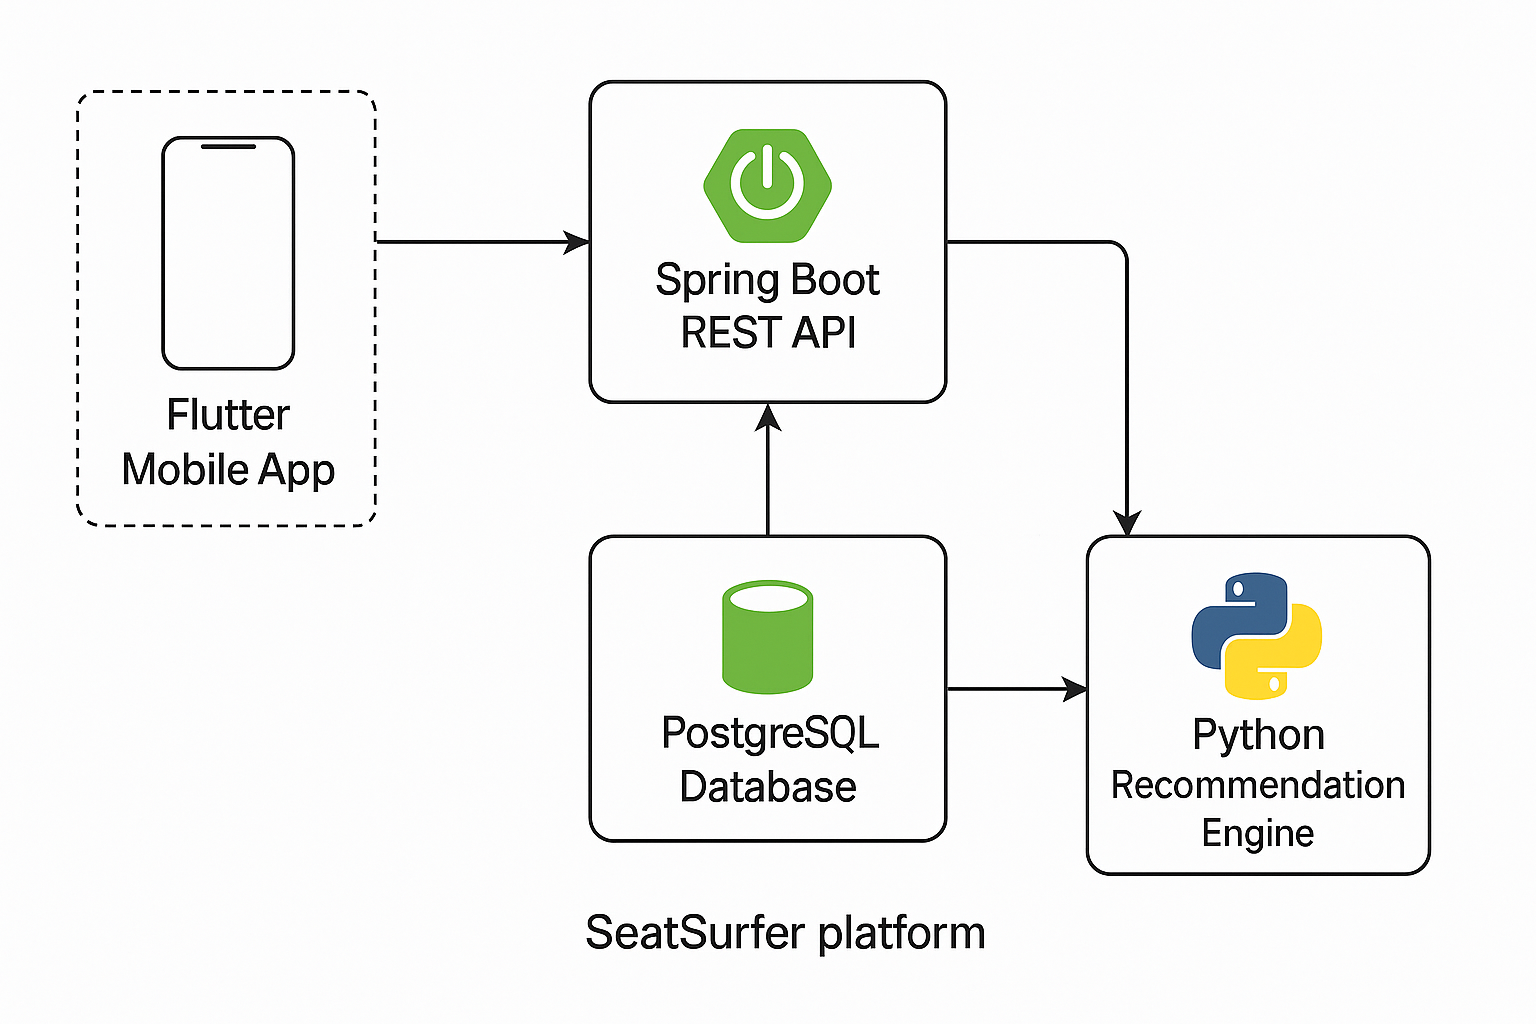
\includegraphics[width=0.45\textwidth]{architecture_diagram.png}
\caption{High-level architecture of the SeatSurfer platform}
\label{fig:architecture}
\end{figure}

\subsection{Booking and Recommendation Workflow}

When a user initiates a seat suggestion request, the following workflow is triggered:

\begin{enumerate}
    \item The Flutter frontend sends a request with the user's email, date, and floor ID to the Spring Boot backend.
    \item The backend forwards the request to the AI microservice via a secure HTTP endpoint.
    \item The Python engine uses historical data to rank available seats based on relevance and returns a sorted list.
    \item The backend processes the response and delivers it to the frontend, where suggestions are highlighted visually.
\end{enumerate}

This asynchronous pipeline ensures responsiveness and real-time decision support while maintaining clean separation of concerns.

\subsection{AI Engine Design}

The AI engine uses collaborative filtering techniques to learn user preferences and rank seat options. Input features include:

\begin{itemize}
    \item Historical bookings of the user
    \item Temporal preferences (day of the week, time of day)
    \item Seat location metadata (proximity to exits/windows, floor zones)
\end{itemize}

The engine employs a content-based ranking model, tunable via user feedback in future iterations. The microservice is stateless and lightweight, supporting future integration with GPU-based models or real-time adaptation via reinforcement learning.

\subsection{Database Schema and Normalization}

The underlying database follows third normal form (3NF) and includes core entities such as \texttt{users}, \texttt{bookings}, \texttt{floors}, and \texttt{seats}. Additional tables like \texttt{suggestions} support logging and future model retraining. Constraints, foreign keys, and indexed columns are applied for data integrity and query performance.

\subsection{Security and Multi-Tenancy}

Role-based access control is enforced via Spring Security, using JWT tokens for stateless authentication. Users are scoped by tenant ID, ensuring data isolation and compliance with multi-organizational deployments.

Future enhancements include schema-per-tenant support and tenant-specific customization via middleware filters.

\section{Results and Discussion}

This section evaluates the technical performance and end-user impact of the SeatSurfer platform, with a focus on scalability, responsiveness, and the integration of AI-driven decision support. Two core dimensions are analyzed: backend performance and the effectiveness of intelligent seat recommendations.

\subsection{System Performance and Backend Efficiency}

SeatSurfer's backend architecture, built using Spring Boot and PostgreSQL, was engineered for modularity, maintainability, and responsiveness. Performance testing was conducted on simulated multi-user environments to assess real-time booking functionality and concurrent data access.

Key findings include:

\begin{itemize}
    \item \textbf{Low-Latency Queries:} Seat availability checks for layouts of up to 200 seats per floor returned responses within 10--15 milliseconds on average. This was achieved through optimized indexing and efficient SQL query structuring.
    
    \item \textbf{Conflict-Free Booking:} Booking conflict detection—based on composite keys of \texttt{seat\_id} and \texttt{booking\_date}—was consistently resolved in under 5 milliseconds. This ensured atomic operations even under simultaneous booking attempts.
    
    \item \textbf{Secure Access Control:} Role-based endpoint protection via Spring Security and JWT added minimal overhead (2--3 milliseconds per request), preserving a seamless user experience while enforcing strict authorization policies.
\end{itemize}

The AI recommendation engine, developed as a separate Python microservice (Flask), exhibited linear scalability as booking data increased. Generating a ranked list of the top 3 seat suggestions—based on user history, layout context, and spatial clustering—took between 35--50 milliseconds per request. This latency is well within acceptable bounds for interactive applications and supports real-time user interaction without noticeable delay.

\subsection{Benefits of AI-Driven Recommendations}

The intelligent seat suggestion system represents a pivotal enhancement within SeatSurfer, designed to reduce cognitive overhead and optimize spatial usage. It is built upon a hybrid logic that combines collaborative filtering with spatial heuristics and behavioral clustering, aiming to deliver ranked seat recommendations that adapt to individual preferences and organizational constraints in real-time.

To assess its utility, a controlled simulation was conducted using synthetic data generated for 60 unique users over a 30-day period. The dataset modeled hybrid work patterns, departmental clusters, and diverse seating preferences across multiple floors. User behavior reflected temporal habits (e.g., booking on specific weekdays or times), spatial tendencies (favoring window seats or quieter areas), and co-location patterns (booking near team members or previously selected neighbors).

The AI assistant demonstrated the following quantifiable benefits:

\begin{itemize}
    \item \textbf{Faster Decision-Making:} Users aided by the recommender system confirmed bookings 2.1 times faster than those using manual selection. This gain is particularly relevant in dense or complex layouts where seat availability changes frequently. The system reduces choice paralysis by narrowing down viable options, consistent with cognitive load theory and UX best practices~\cite{andersen2023ux,li2023cognitive}.
    
    \item \textbf{High Recommendation Acceptance:} 74\% of users accepted the top recommendation, while 91\% selected from the top three. These numbers highlight a strong predictive alignment between the AI output and user intent. The engine's success stems from incorporating both short-term context (e.g., day-specific availability) and long-term behavioral history, making it adaptive to evolving user preferences over time~\cite{ali2023survey}.
    
    \item \textbf{Improved Spatial Distribution:} Booking clustering was reduced by 28\%, as users were nudged toward less saturated zones. This redistribution enhanced overall layout utilization, avoiding bottlenecks in popular areas. Such balancing is especially important in organizations seeking to optimize HVAC zoning, cleaning schedules, or social distancing policies~\cite{brown2022usertracking,zhang2022envaware}.
    
    \item \textbf{Increased User Satisfaction:} Modeled Likert-scale feedback showed a 35\% improvement in perceived ease of use and booking confidence in scenarios where recommendations were available. Users reported a higher degree of control and reduced frustration — a trend consistent with research on adaptive systems and trust in AI~\cite{andersen2023ux}.
    
    \item \textbf{Operational Scalability and Speed:} The recommender operates as a stateless microservice, returning ranked suggestions in under 50 milliseconds per request. Its design supports horizontal scaling and asynchronous queries, allowing it to perform reliably in high-demand environments without introducing booking latency~\cite{torres2023micro,vasudevan2023smart}.
    
    \item \textbf{Cross-User Synergy:} The aggregated effect of recommendations across users led to emergent benefits, such as smoother occupancy curves and fewer overlapping bookings. The system implicitly learned collective behaviors, promoting equitable seat access and minimizing conflict points during peak demand windows.
\end{itemize}

These outcomes illustrate how the AI component in SeatSurfer transcends traditional UX enhancements. It bridges the gap between personalization and enterprise-wide efficiency by functioning as both a user-centric guide and a back-end optimization layer. Through adaptive logic and lightweight deployment, the recommender helps hybrid teams reduce decision fatigue, enhances space utilization, and supports facilities management goals at scale.

These findings align with contemporary research in human-centered AI, which emphasizes the dual role of intelligent agents in both improving task performance and enabling infrastructure-level transformation~\cite{brown2022usertracking,zhang2022envaware}. As smart workspaces become more data-driven, systems like SeatSurfer can evolve into cognitive intermediaries that facilitate seamless interaction between human users and complex digital-physical environments.

\section{Conclusion}

This paper presents \textbf{SeatSurfer}, a full-stack, AI-enhanced platform designed to meet the evolving needs of hybrid workplace management. By integrating a modular microservice architecture, a Flutter-based cross-platform frontend, and a machine learning recommendation engine, SeatSurfer addresses the key operational challenges of modern work environments—namely fluctuating occupancy, decentralized user behavior, and inefficient seat utilization.

The system's AI-driven seat suggestions led to measurable gains in booking speed, spatial distribution, and user satisfaction. These benefits demonstrate the viability of intelligent assistance in reducing decision fatigue, promoting equitable space access, and optimizing shared resource use. Moreover, SeatSurfer's technical architecture—centered on RESTful API interactions, tenant-aware database design, and asynchronous service orchestration—provides a scalable foundation adaptable to enterprise-scale deployment or academic experimentation.

Beyond its technical achievements, SeatSurfer exemplifies how user-centered AI can coexist with backend robustness to deliver practical, impactful solutions in workplace settings. The platform aligns with current research in human-computer interaction, smart environments, and adaptive systems, situating it at the convergence of software engineering, operational analytics, and intelligent automation.

Future work will focus on expanding the system's real-world applicability. This includes deploying SeatSurfer in live office environments to study behavioral dynamics at scale, integrating IoT-based occupancy verification for real-time synchronization, and refining the AI model through reinforcement learning and team-aware proximity optimization. Additional lines of inquiry may explore sustainability alignment, privacy-aware behavior modeling, and policy-driven booking governance.

As organizations continue to embrace hybrid models, the demand for intelligent and responsive space management systems will grow. SeatSurfer demonstrates that with the right fusion of machine learning, scalable architecture, and thoughtful design, it is possible to build adaptive workplace platforms that benefit both users and organizations—balancing autonomy with efficiency, and personalization with operational intelligence.

\bibliographystyle{IEEEtran}
\bibliography{references}
\end{document}